\chapter{विद्युत-ऋणात्मकता, ध्रुवता और अंतराआण्विक बल}\label{ch:g11:polarity-and-cohesion}

एक छिपकली खिड़की के शीशे पर ऊपर दौड़ जाती है और एक ही उँगली के सहारे
काँच से लटक जाती है, बिना किसी गोंद और बिना किसी चूषण-कप के। पानी का \omterm{def:g7:atoms-and-molecules:molecule}{अणु},
\ce{H2O}, हाइड्रोजन सल्फ़ाइड के \omterm{def:g7:atoms-and-molecules:molecule}{अणु}, \ce{H2S}, से हल्का है, फिर भी पानी
\qty{100}{\celsius} पर उबलता है जबकि हाइड्रोजन सल्फ़ाइड
\qty{-60}{\celsius} तक गैस रहता है। दोनों कहानियाँ एक ही बात के बारे में हैं: वे बल
जो \omterm{def:g7:atoms-and-molecules:molecule}{अणुओं} को एक-दूसरे से, और दूसरी चीज़ों से, जोड़े रखते हैं। वे \omterm{def:g7:atoms-and-molecules:molecule}{अणु} के भीतर के
\omterm{def:g10:lewis-and-shape:covalent-bond}{सहसंयोजी आबंधों} से कहीं दुर्बल हैं, पर वही तय करते हैं कि कमरे के ताप पर कोई पदार्थ
गैस है, द्रव है या ठोस, और यह भी कि छिपकली
गिरती है या नहीं।

\begin{recall}
\omterm{def:g10:lewis-and-shape:covalent-bond}{सहसंयोजी आबंध} दो \omterm{def:g7:atoms-and-molecules:atom}{परमाणुओं} द्वारा साझा किया गया \omterm{def:g9:inside-the-atom:nucleus}{इलेक्ट्रॉनों} का एक युग्म है; \omterm{def:g10:lewis-and-shape:lewis-structure}{लुइस
संरचनाएँ} \omterm{def:g10:lewis-and-shape:lone-pair}{आबंधी युग्म} और \omterm{def:g10:lewis-and-shape:lone-pair}{एकाकी युग्म} दिखाती हैं, और केंद्रीय \omterm{def:g7:atoms-and-molecules:atom}{परमाणु} के चारों ओर
के युग्म \omterm{def:g7:atoms-and-molecules:molecule}{अणु} की आकृति तय करते हैं
(\cref{ch:g10:lewis-and-shape})। \omterm{def:g9:ions:ion}{आयनों} पर आवेश होता है; आयनिक ठोस में
धनात्मक और ऋणात्मक \omterm{def:g9:ions:ion}{आयन} एक-दूसरे को आकर्षित करते हैं (\cref{ch:g9:ions})।
\end{recall}

\begin{omfigure}
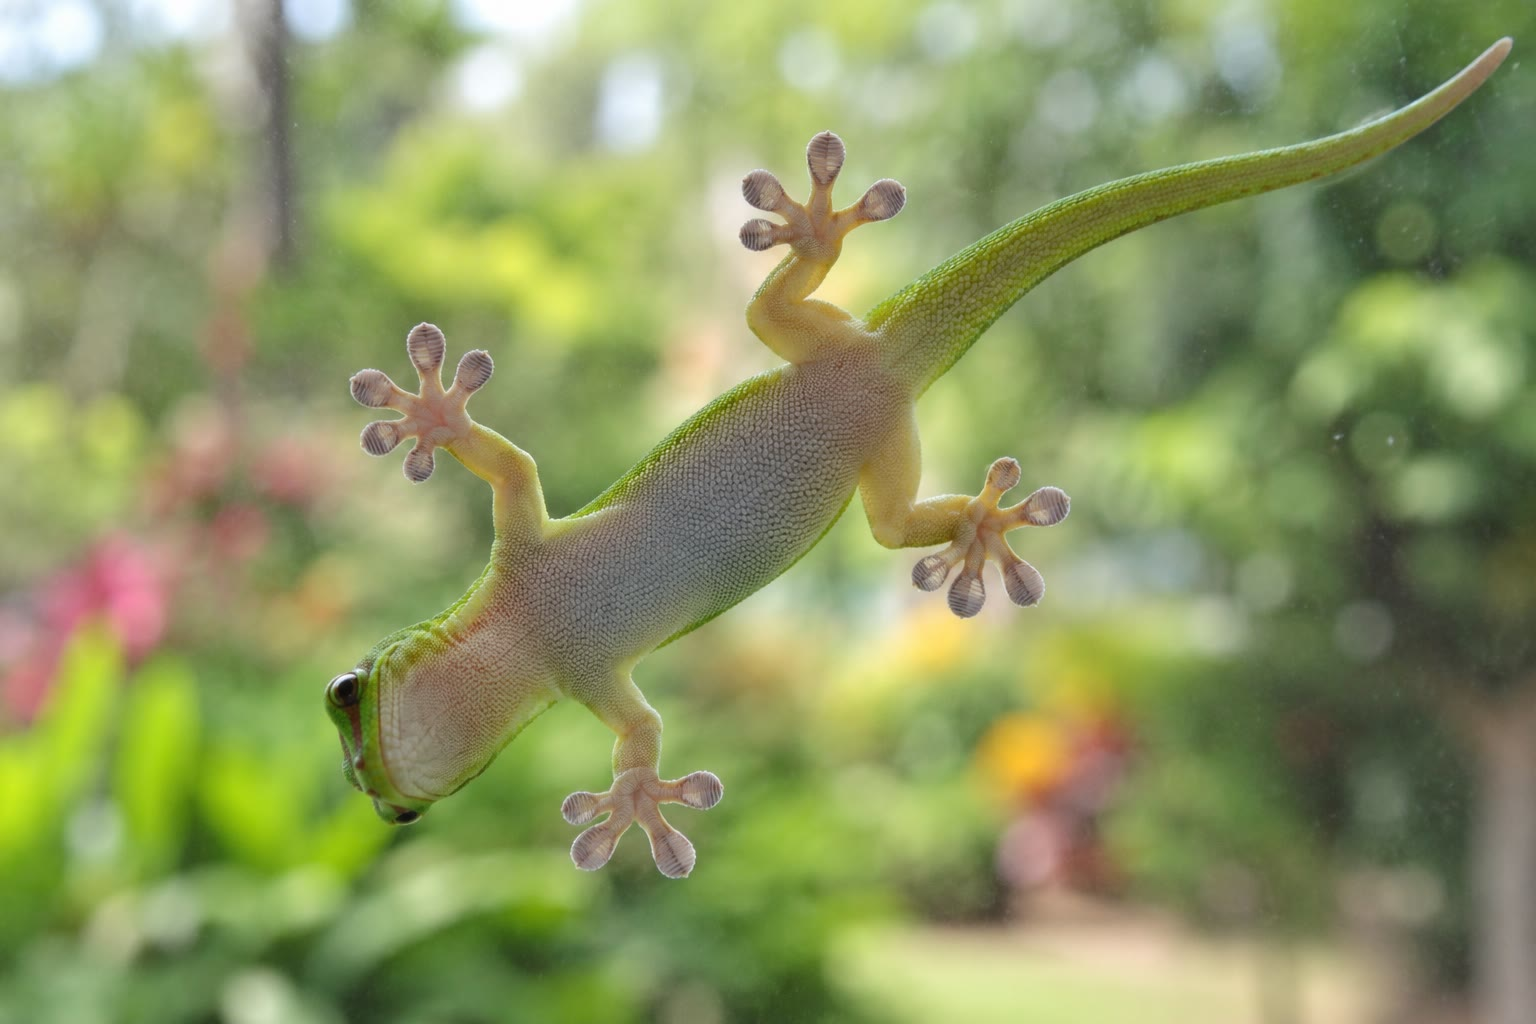
\includegraphics[width=0.5\linewidth]{images/book1/ai/g11-gecko-glass.jpg}

{\small काँच के शीशे पर एक छिपकली: उसकी उँगलियों की गद्दियाँ \omterm{def:g7:atoms-and-molecules:molecule}{अणुओं} के बीच के
बलों से टिकी रहती हैं।}
\end{omfigure}

\section{विद्युत-ऋणात्मकता}

\begin{definition}[विद्युत-ऋणात्मकता]\label{def:g11:polarity-and-cohesion:electronegativity}
किसी तत्व की \emph{विद्युत-ऋणात्मकता}\index{विद्युत-ऋणात्मकता} मापती है कि
\omterm{def:g7:atoms-and-molecules:molecule}{अणु} में उसके \omterm{def:g7:atoms-and-molecules:atom}{परमाणु} अपने द्वारा साझा किए गए आबंधों के \omterm{def:g9:inside-the-atom:nucleus}{इलेक्ट्रॉनों} को कितनी
तीव्रता से आकर्षित करते हैं। यह एक मात्रकरहित संख्या है; सामान्य पैमाने पर यह
लगभग 0.8 से लगभग 4 तक जाती है।
\end{definition}

\begin{omfigure}
% ledger: en:H, en:Li, en:Be, en:B, en:C, en:N, en:O, en:F, en:Na, en:Mg, en:Al, en:Si, en:P, en:S, en:Cl, en:K, en:Ca
\omperiodictable[upto=20, f block=false, cell=0.9cm, values={H/2.20,
  Li/0.98, Be/1.57, B/2.04, C/2.55, N/3.04, O/3.44, F/3.98, Na/0.93,
  Mg/1.31, Al/1.61, Si/1.90, P/2.19, S/2.58, Cl/3.16, K/0.82, Ca/1.00},
  highlight={F,O,N,Cl}]

{\small पहले बीस तत्वों की \omterm{def:g11:polarity-and-cohesion:electronegativity}{विद्युत-ऋणात्मकताएँ} (पॉलिंग पैमाना;
हीलियम, नियॉन और आर्गन के लिए कोई मान नहीं दिया गया, क्योंकि वे यहाँ कोई आबंध
नहीं बनाते)। उभारे गए: चार सबसे अधिक विद्युत-ऋणात्मक तत्व।}
\end{omfigure}

\begin{proposition}[सारणी में प्रवृत्तियाँ]\label{prop:g11:polarity-and-cohesion:trends}
% ledger: en:F, en:Li, en:Cl, en:K
\omterm{def:g11:polarity-and-cohesion:electronegativity}{विद्युत-ऋणात्मकता} \omterm{def:g9:periodic-table-first-look:period}{आवर्त} में बाएँ से दाएँ बढ़ती है और समूह में ऊपर से नीचे
घटती है। फ़्लुओरीन (3.98) सबसे अधिक विद्युत-ऋणात्मक तत्व है; \omterm{def:g10:electron-shells:family}{क्षार धातुएँ} सबसे
कम हैं (लिथियम 0.98,
पोटैशियम 0.82)।
\end{proposition}

\begin{proof}
सारणी पर पढ़िए: \omterm{def:g9:periodic-table-first-look:period}{आवर्त} 2 में $0.98 < 1.57 < 2.04 < 2.55 < 3.04 <
3.44 < 3.98$; \omterm{def:g9:periodic-table-first-look:period}{समूह} 17 में नीचे, फ़्लुओरीन $3.98$ क्लोरीन
$3.16$ से ऊपर है; \omterm{def:g9:periodic-table-first-look:period}{समूह} 1 में नीचे, $2.20$, $0.98$, $0.93$, $0.82$। (ऐसा क्यों है,
यह विश्वविद्यालय के प्रथम वर्ष के खंड में समझाया गया है।)
\end{proof}

\begin{history}[पॉलिंग का पैमाना, 1932]
रसायनज्ञ लाइनस पॉलिंग ने 1932 में अलग-अलग \omterm{def:g7:atoms-and-molecules:atom}{परमाणुओं} के बीच के आबंधों की ऊर्जाओं से
\omterm{def:g11:polarity-and-cohesion:electronegativity}{विद्युत-ऋणात्मकता} का पहला पैमाना बनाया। उन्होंने फ़्लुओरीन को सबसे बड़ा मान दिया,
और इस अध्याय में इस्तेमाल हुआ पैमाना आज भी उन्हीं के नाम से
जाना जाता है।
\end{history}

\section{ध्रुवीय आबंध और ध्रुवीय अणु}

\begin{definition}[ध्रुवीय आबंध, आंशिक आवेश]\label{def:g11:polarity-and-cohesion:polar-bond}
अलग-अलग \omterm{def:g11:polarity-and-cohesion:electronegativity}{विद्युत-ऋणात्मकताओं} वाले दो \omterm{def:g7:atoms-and-molecules:atom}{परमाणुओं} के बीच का \omterm{def:g10:lewis-and-shape:covalent-bond}{सहसंयोजी आबंध}
\emph{ध्रुवीय आबंध}\index{ध्रुवीय आबंध} है: साझा युग्म अधिक विद्युत-ऋणात्मक
\omterm{def:g7:atoms-and-molecules:atom}{परमाणु} के अधिक पास होता है। उस \omterm{def:g7:atoms-and-molecules:atom}{परमाणु} पर एक छोटा ऋणात्मक
\emph{आंशिक आवेश}\index{आंशिक आवेश} होता है, जिसे $\delta^-$ लिखा जाता है, और
दूसरे \omterm{def:g7:atoms-and-molecules:atom}{परमाणु} पर उतना ही धनात्मक आंशिक आवेश, $\delta^+$।
\end{definition}

\begin{proposition}[आबंध कब ध्रुवीय होता है?]\label{prop:g11:polarity-and-cohesion:polar-bond}
% ledger: en:C, en:H, en:O, en:Na, en:Cl
दो समान \omterm{def:g7:atoms-and-molecules:atom}{परमाणुओं} के बीच का आबंध ध्रुवीय नहीं होता। अलग-अलग \omterm{def:g7:atoms-and-molecules:atom}{परमाणुओं} के बीच
\omterm{def:g11:polarity-and-cohesion:electronegativity}{विद्युत-ऋणात्मकताओं} का अंतर जितना अधिक, आबंध उतना अधिक ध्रुवीय; मोटे नियम के
तौर पर लगभग 0.4 से कम अंतर (जैसे
\ce{C-H}, $2.55 - 2.20 = 0.35$) को अध्रुवीय माना जाता है। जब अंतर बहुत
बड़ा हो (जैसे Na और Cl, $3.16 - 0.93 = 2.23$), तो \omterm{def:g9:inside-the-atom:nucleus}{इलेक्ट्रॉन} साझा नहीं होते,
बल्कि स्थानांतरित होते हैं: यौगिक आयनिक है।
\end{proposition}

\begin{proof}
स्वीकृत: यह \omterm{def:g11:polarity-and-cohesion:electronegativity}{विद्युत-ऋणात्मकता} की परिभाषा से निकलता है, और सीमाएँ
परिपाटियाँ हैं।
\end{proof}

\begin{definition}[ध्रुवीय और अध्रुवीय अणु]\label{def:g11:polarity-and-cohesion:polar-molecule}
कोई \omterm{def:g7:atoms-and-molecules:molecule}{अणु} \emph{ध्रुवीय अणु}\index{ध्रुवीय अणु} है अगर उसके धनात्मक \omterm{def:g11:polarity-and-cohesion:polar-bond}{आंशिक
आवेशों} का केंद्र और उसके ऋणात्मक \omterm{def:g11:polarity-and-cohesion:polar-bond}{आंशिक आवेशों} का केंद्र संपाती न हों; अगर
वे संपाती हों, तो वह
\emph{अध्रुवीय अणु}\index{अध्रुवीय अणु} है।
\end{definition}

\begin{method}[क्या अणु ध्रुवीय है?]\label{met:g11:polarity-and-cohesion:polar}
\begin{enumerate}
  \item \omterm{def:g10:lewis-and-shape:lewis-structure}{लुइस संरचना} बनाइए और \omterm{def:g7:atoms-and-molecules:molecule}{अणु} की आकृति ज्ञात कीजिए।
  \item \omterm{def:g11:polarity-and-cohesion:polar-bond}{ध्रुवीय आबंधों} पर $\delta^+$ और $\delta^-$ अंकित कीजिए।
  \item अगर कोई \omterm{def:g11:polarity-and-cohesion:polar-bond}{ध्रुवीय आबंध} नहीं है, तो \omterm{def:g7:atoms-and-molecules:molecule}{अणु} अध्रुवीय है। नहीं तो,
        आकृति देखिए: अगर \omterm{def:g11:polarity-and-cohesion:polar-bond}{ध्रुवीय आबंध} केंद्र के चारों ओर सममित रूप से सजे हैं,
        तो उनके प्रभाव निरस्त हो जाते हैं और \omterm{def:g7:atoms-and-molecules:molecule}{अणु}
        अध्रुवीय है; नहीं तो, वह ध्रुवीय है।
\end{enumerate}
\end{method}

\begin{omfigure}
\begin{tikzpicture}[font=\small]
  % water
  \begin{scope}
    \node[aO] (o) at (0,0) {};
    \node[aH] (h1) at (-0.82,-0.6) {};
    \node[aH] (h2) at (0.82,-0.6) {};
    \begin{scope}[on background layer]
      \draw[bond] (o.center) -- (h1.center); \draw[bond] (o.center) -- (h2.center);
    \end{scope}
    \node[omThm] at (0,0.55) {$2\delta^-$};
    \node[omDef] at (-1.22,-0.5) {$\delta^+$};
    \node[omDef] at (1.22,-0.5) {$\delta^+$};
    \fill[omDef] (0,-0.6) circle (0.06);
    \fill[omThm] (0,0) circle (0.06);
    \draw[densely dotted, black!60] (-0.82,-0.6) -- (0.82,-0.6);
    \draw[<-, black!60] (0.08,-0.64) -- (1.55,-1.05) node[right, align=left,
      font=\footnotesize] {$\delta^+$ का\\ केंद्र};
    \node[align=center, anchor=north] at (0,-1.8) {पानी: मुड़ा हुआ, \textbf{ध्रुवीय}};
  \end{scope}
  % carbon dioxide
  \begin{scope}[xshift=6cm]
    \node[aO] (o1) at (-1.15,0) {};
    \node[aC] (c) at (0,0) {};
    \node[aO] (o2) at (1.15,0) {};
    \begin{scope}[on background layer]
      \draw[bond, double, double distance=1.6pt] (o1.center) -- (c.center);
      \draw[bond, double, double distance=1.6pt] (c.center) -- (o2.center);
    \end{scope}
    \node[omThm] at (-1.15,0.55) {$\delta^-$};
    \node[omThm] at (1.15,0.55) {$\delta^-$};
    \node[omDef] at (0,0.55) {$2\delta^+$};
    \draw[->, omProp, thick] (-0.25,-0.45) -- (-1.0,-0.45);
    \draw[->, omProp, thick] (0.25,-0.45) -- (1.0,-0.45);
    \node[align=center, anchor=north] at (0,-1.8) {कार्बन डाइऑक्साइड: रैखिक,\\
      \textbf{अध्रुवीय}};
  \end{scope}
\end{tikzpicture}

{\small पानी में मुड़ी हुई आकृति धनात्मक \omterm{def:g11:polarity-and-cohesion:polar-bond}{आंशिक आवेशों} के केंद्र (हाइड्रोजन
\omterm{def:g7:atoms-and-molecules:atom}{परमाणुओं} के बीच) को ऑक्सीजन \omterm{def:g7:atoms-and-molecules:atom}{परमाणु} के नीचे रखती है: \omterm{def:g7:atoms-and-molecules:molecule}{अणु}
ध्रुवीय है। कार्बन डाइऑक्साइड में दोनों \omterm{def:g11:polarity-and-cohesion:polar-bond}{ध्रुवीय आबंध} विपरीत दिशाओं में खींचते हैं
(तीर) और निरस्त हो जाते हैं: आवेशों के केंद्र
कार्बन \omterm{def:g7:atoms-and-molecules:atom}{परमाणु} पर संपाती होते हैं।}
\end{omfigure}


\begin{example}[चार अणु]\label{ex:g11:polarity-and-cohesion:four}
हाइड्रोजन क्लोराइड \ce{HCl} में एक \omterm{def:g11:polarity-and-cohesion:polar-bond}{ध्रुवीय आबंध} है और वह ध्रुवीय है, क्लोरीन
$\delta^-$। अमोनिया \ce{NH3}, तीन ध्रुवीय \ce{N-H} आबंधों का एक पिरामिड,
ध्रुवीय है, नाइट्रोजन $\delta^-$। मेथेन \ce{CH4} में केवल लगभग अध्रुवीय
\ce{C-H} आबंध हैं: अध्रुवीय। टेट्राक्लोरोमेथेन \ce{CCl4} में चार ध्रुवीय
\ce{C-Cl} आबंध हैं, पर एक नियमित चतुष्फलक के कोनों पर: उनके
प्रभाव निरस्त हो जाते हैं और \omterm{def:g7:atoms-and-molecules:molecule}{अणु} अध्रुवीय है।
\end{example}

\section{वान्डरवाल्स अन्योन्यक्रियाएँ}

\begin{definition}[वान्डरवाल्स अन्योन्यक्रिया]\label{def:g11:polarity-and-cohesion:van-der-waals}
\emph{वान्डरवाल्स अन्योन्यक्रिया}\index{वान्डरवाल्स अन्योन्यक्रिया}
पड़ोसी \omterm{def:g7:atoms-and-molecules:molecule}{अणुओं} के बीच का एक दुर्बल आकर्षण है, जो सभी \omterm{def:g7:atoms-and-molecules:molecule}{अणुओं} के बीच होता है,
ध्रुवीय हों या नहीं: हर \omterm{def:g7:atoms-and-molecules:molecule}{अणु} के \omterm{def:g9:inside-the-atom:nucleus}{इलेक्ट्रॉन} लगातार
घूमते रहते हैं, और एक \omterm{def:g7:atoms-and-molecules:molecule}{अणु} के क्षणिक असमान आवेश उसके पड़ोसियों के क्षणिक आवेशों
को आकर्षित करते हैं। \omterm{def:g11:polarity-and-cohesion:polar-molecule}{ध्रुवीय अणुओं} के बीच स्थायी \omterm{def:g11:polarity-and-cohesion:polar-bond}{आंशिक
आवेश} एक और आकर्षण जोड़ देते हैं।
\end{definition}


\begin{proposition}[बड़े अणु अधिक आकर्षित करते हैं]\label{prop:g11:polarity-and-cohesion:size}
\omterm{def:g11:polarity-and-cohesion:van-der-waals}{वान्डरवाल्स अन्योन्यक्रियाएँ} \omterm{def:g7:atoms-and-molecules:molecule}{अणुओं} के आकार के साथ, यानी
उनके \omterm{def:g9:inside-the-atom:nucleus}{इलेक्ट्रॉनों} की संख्या के साथ, बढ़ती हैं; मिलते-जुलते \omterm{def:g7:atoms-and-molecules:molecule}{अणुओं} में
बड़े \omterm{def:g7:atoms-and-molecules:molecule}{अणुओं} के गलन और क्वथन ताप अधिक होते हैं।
\end{proposition}

\begin{proof}
स्वीकृत: बड़ा \omterm{def:g9:inside-the-atom:nucleus}{इलेक्ट्रॉन} बादल अधिक आसानी से विकृत होता है, इसलिए उसके
क्षणिक आवेश बड़े होते हैं, और उसका अपने पड़ोसियों से संपर्क
अधिक होता है।
\end{proof}

\begin{example}[हैलोजन]\label{ex:g11:polarity-and-cohesion:halogens}
% ledger: bp:F2, bp:Cl2, bp:Br2, bp:I2 (K values converted)
\omterm{def:g7:atoms-and-molecules:molecule}{अणु} \ce{F2}, \ce{Cl2}, \ce{Br2}, \ce{I2} सभी अध्रुवीय हैं और
उत्तरोत्तर बड़े हैं। उनके क्वथन ताप उनके साथ बढ़ते हैं:
\qty{-188}{\celsius}, \qty{-34}{\celsius}, \qty{59}{\celsius} और
\qty{184}{\celsius}। कमरे के ताप पर फ़्लुओरीन और क्लोरीन
गैसें हैं, ब्रोमीन द्रव है, आयोडीन ठोस।
\end{example}

\begin{remark}[छिपकली]\label{rem:g11:polarity-and-cohesion:gecko}
एक अकेली \omterm{def:g11:polarity-and-cohesion:van-der-waals}{वान्डरवाल्स अन्योन्यक्रिया} बहुत छोटी होती है, पर वे जुड़ती जाती हैं।
छिपकली की उँगलियों की गद्दियाँ सूक्ष्म रोमों के घने ग़लीचे से ढकी होती हैं,
जिनमें से हर एक और भी बारीक सिरों में बँटा होता है, जो काँच के इतने पास आ जाते हैं
कि \omterm{def:g11:polarity-and-cohesion:van-der-waals}{वान्डरवाल्स अन्योन्यक्रियाएँ} एक बहुत बड़े कुल क्षेत्रफल पर काम करती हैं।
\end{remark}

\section{हाइड्रोजन आबंध}

\begin{definition}[हाइड्रोजन आबंध]\label{def:g11:polarity-and-cohesion:hydrogen-bond}
\emph{हाइड्रोजन आबंध}\index{हाइड्रोजन आबंध} किसी बहुत विद्युत-ऋणात्मक \omterm{def:g7:atoms-and-molecules:atom}{परमाणु}
(नाइट्रोजन, ऑक्सीजन या फ़्लुओरीन) से आबंधित हाइड्रोजन \omterm{def:g7:atoms-and-molecules:atom}{परमाणु}, जिस पर स्पष्ट
$\delta^+$ होता है, और किसी दूसरे नाइट्रोजन, ऑक्सीजन या फ़्लुओरीन \omterm{def:g7:atoms-and-molecules:atom}{परमाणु} के \omterm{def:g10:lewis-and-shape:lone-pair}{एकाकी
युग्म} के बीच का आकर्षण है, जो अक्सर किसी पड़ोसी \omterm{def:g7:atoms-and-molecules:molecule}{अणु} पर होता है। इसे
डैश वाली रेखा से बनाया जाता है, और इसमें शामिल तीनों \omterm{def:g7:atoms-and-molecules:atom}{परमाणु} लगभग एक सीधी
रेखा में होते हैं।
\end{definition}

\begin{omfigure}
\begin{tikzpicture}[font=\small]
  % central water molecule and four neighbours, H-bonds dashed
  \newcommand{\water}[4]{% name, x, y, rotation
    \begin{scope}[shift={(#2,#3)}, rotate=#4]
      \node[aO] (#1o) at (0,0) {};
      \node[aH] (#1a) at (-0.6,-0.45) {};
      \node[aH] (#1b) at (0.6,-0.45) {};
    \end{scope}
    \begin{scope}[on background layer]
      \draw[bond] (#1o.center) -- (#1a.center); \draw[bond] (#1o.center) -- (#1b.center);
    \end{scope}}
  \water{m}{0}{0}{0}
  \water{p}{-1.62}{-1.215}{0}
  \water{q}{1.62}{-1.215}{0}
  \water{r}{-1.435}{1.435}{-8.13}
  \water{s}{1.435}{1.435}{8.13}
  % H-bonds: m's H to p's O and q's O; r's and s's H to m's O
  \draw[dashed, omDef, thick] (ma) -- (po);
  \draw[dashed, omDef, thick] (mb) -- (qo);
  \draw[dashed, omDef, thick] (rb) -- (mo);
  \draw[dashed, omDef, thick] (sa) -- (mo);
\end{tikzpicture}

{\small द्रव पानी में एक पानी के \omterm{def:g7:atoms-and-molecules:molecule}{अणु} के चारों ओर \omterm{def:g11:polarity-and-cohesion:hydrogen-bond}{हाइड्रोजन आबंध} (डैश वाले):
उसके दोनों हाइड्रोजन \omterm{def:g7:atoms-and-molecules:atom}{परमाणु} दो पड़ोसियों के ऑक्सीजन \omterm{def:g7:atoms-and-molecules:atom}{परमाणुओं} से आबंधित होते हैं, और
उसके ऑक्सीजन \omterm{def:g7:atoms-and-molecules:atom}{परमाणु} के दोनों \omterm{def:g10:lewis-and-shape:lone-pair}{एकाकी युग्म} दो और \omterm{def:g7:atoms-and-molecules:molecule}{अणुओं} के हाइड्रोजन \omterm{def:g7:atoms-and-molecules:atom}{परमाणुओं} को
ग्रहण करते हैं।}
\end{omfigure}


\begin{example}[एथेनॉल और प्रोपेन]\label{ex:g11:polarity-and-cohesion:ethanol}
% ledger: bp:C2H5OH, bp:C3H8 (K values converted)
एथेनॉल, \ce{CH3-CH2-OH} (\qty{46.0}{g/mol}), और प्रोपेन,
\ce{CH3-CH2-CH3} (\qty{44.0}{g/mol}), के \omterm{def:g7:atoms-and-molecules:molecule}{अणु} लगभग एक ही
आकार के हैं। फिर भी एथेनॉल \qty{78}{\celsius} पर उबलता है और प्रोपेन
\qty{-42}{\celsius} पर। एथेनॉल के \omterm{def:g7:atoms-and-molecules:molecule}{अणु}, अपने \ce{O-H} समूह के साथ, आपस में
\omterm{def:g11:polarity-and-cohesion:hydrogen-bond}{हाइड्रोजन आबंध} बनाते हैं; प्रोपेन के \omterm{def:g7:atoms-and-molecules:molecule}{अणु} नहीं बना सकते।
\end{example}

\section{ठोसों और द्रवों का संसंजन}

\begin{definition}[आण्विक ठोस]\label{def:g11:polarity-and-cohesion:molecular-solid}
\emph{आण्विक ठोस}\index{आण्विक ठोस} ऐसे \omterm{def:g7:atoms-and-molecules:molecule}{अणुओं} से बना ठोस है जो
\omterm{def:g11:polarity-and-cohesion:van-der-waals}{वान्डरवाल्स अन्योन्यक्रियाओं} से और, जहाँ संभव हो, \omterm{def:g11:polarity-and-cohesion:hydrogen-bond}{हाइड्रोजन आबंधों} से
एक-दूसरे से जुड़े रहते हैं। बर्फ़, ठोस आयोडीन और चीनी आण्विक
ठोस हैं।
\end{definition}

\begin{proposition}[संसंजन और अवस्था-परिवर्तन]\label{prop:g11:polarity-and-cohesion:cohesion}
किसी पदार्थ के कणों के बीच आकर्षण जितना प्रबल होता है, उसके गलन और क्वथन ताप
उतने ही ऊँचे होते हैं। प्रबलता के बढ़ते क्रम में:
\omterm{def:g11:polarity-and-cohesion:van-der-waals}{वान्डरवाल्स अन्योन्यक्रियाएँ}, \omterm{def:g11:polarity-and-cohesion:hydrogen-bond}{हाइड्रोजन आबंध}, और आयनिक ठोस के \omterm{def:g9:ions:ion}{आयनों} के बीच
का आकर्षण।
\end{proposition}

\begin{proof}
स्वीकृत: पिघलना और उबलना कणों को इन आकर्षणों के विरुद्ध अलग खींचता है,
जिसके लिए आकर्षण प्रबल होने पर अधिक ऊर्जा, यानी अधिक ऊँचा ताप,
चाहिए।
\end{proof}

\begin{example}[तीन ठोस]\label{ex:g11:polarity-and-cohesion:three}
% ledger: mp:NaCl, mp:water
सोडियम क्लोराइड, एक आयनिक ठोस, \qty{801}{\celsius} पर पिघलता है; बर्फ़, जो
\omterm{def:g11:polarity-and-cohesion:hydrogen-bond}{हाइड्रोजन आबंधों} से जुड़ी है, \qty{0}{\celsius} पर; ठोस मेथेन, जो छोटे \omterm{def:g7:atoms-and-molecules:molecule}{अणुओं} के बीच
केवल \omterm{def:g11:polarity-and-cohesion:van-der-waals}{वान्डरवाल्स अन्योन्यक्रियाओं} से जुड़ी है,
\qty{-150}{\celsius} से बहुत नीचे।
\end{example}

\begin{omfigure}
\begin{tikzpicture}
\begin{axis}[width=0.6\linewidth, height=7cm, xmin=1.7, xmax=5.3,
    ymin=-190, ymax=120, xtick={2,3,4,5}, xlabel={आवर्त},
    ylabel={क्वथन ताप (\si{\celsius})}, axis lines*=left,
    ymajorgrids, grid style={gray!20}, tick label style={font=\small},
    label style={font=\small},
    legend style={font=\small, at={(1.02,0.5)}, anchor=west, draw=none},
    legend cell align=left]
  % ledger: bp:CH4, bp:SiH4, bp:GeH4, bp:NH3, bp:PH3, bp:AsH3, bp:SbH3, bp:H2O, bp:H2S, bp:H2Se, bp:HF, bp:HCl, bp:HBr, bp:HI (K values converted to degC)
  \addplot[thick, mark=*, black!70] coordinates {(2,-162.2) (3,-112) (4,-88.1)};
  \addplot[thick, mark=square*, omMeth] coordinates {(2,-33.4) (3,-87.8) (4,-62.5) (5,-18.4)};
  \addplot[thick, mark=triangle*, mark size=3pt, omThm] coordinates {(2,100.0) (3,-60.3) (4,-41.3)};
  \addplot[thick, mark=diamond*, mark size=3pt, omDef] coordinates {(2,19.6) (3,-85.1) (4,-66.4) (5,-35.1)};
  \legend{समूह 14 (\ce{CH4} \dots), समूह 15 (\ce{NH3} \dots),
    समूह 16 (\ce{H2O} \dots), समूह 17 (\ce{HF} \dots)}
  \node[font=\footnotesize, anchor=west] at (axis cs:2.05,100) {\ce{H2O}};
  \node[font=\footnotesize, anchor=west] at (axis cs:2.05,19.6) {\ce{HF}};
  \node[font=\footnotesize, anchor=west] at (axis cs:2.05,-33.4) {\ce{NH3}};
  \node[font=\footnotesize, anchor=north west] at (axis cs:2.05,-166) {\ce{CH4}};
\end{axis}
\end{tikzpicture}

{\small \omterm{def:g9:periodic-table-first-look:period}{समूह} 14 से 17 के तत्वों के हाइड्रोजन के साथ यौगिकों के क्वथन ताप।
हर समूह में वे \omterm{def:g7:atoms-and-molecules:molecule}{अणु} के आकार के साथ बढ़ते हैं, सिवाय \omterm{def:g9:periodic-table-first-look:period}{समूह} 15, 16 और 17 के पहले
सदस्य के, जो बहुत अधिक हैं: अमोनिया, पानी और हाइड्रोजन फ़्लुओराइड \omterm{def:g11:polarity-and-cohesion:hydrogen-bond}{हाइड्रोजन आबंध}
बनाते हैं। (जहाँ इस्तेमाल किए गए स्रोत कोई मान नहीं देते, वहाँ कोई मान आलेखित
नहीं किया गया है।)}
\end{omfigure}

\begin{remark}[बर्फ़ और हिम]\label{rem:g11:polarity-and-cohesion:ice}
बर्फ़ में पानी का हर \omterm{def:g7:atoms-and-molecules:molecule}{अणु} चार पड़ोसियों से हाइड्रोजन आबंधित होता है, षट्कोणीय वलयों
के एक खुले जाल में। यह जाल द्रव पानी की तुलना में अधिक ख़ाली जगह छोड़ता है,
जिसमें आबंध लगातार टूटते और फिर बनते रहते हैं: बर्फ़
पानी से कम घनी है और तैरती है। हिम-क्रिस्टलों की छह-भुजा सममिति जाल के
षट्कोणीय वलयों को दर्शाती है।
\end{remark}

\begin{omfigure}
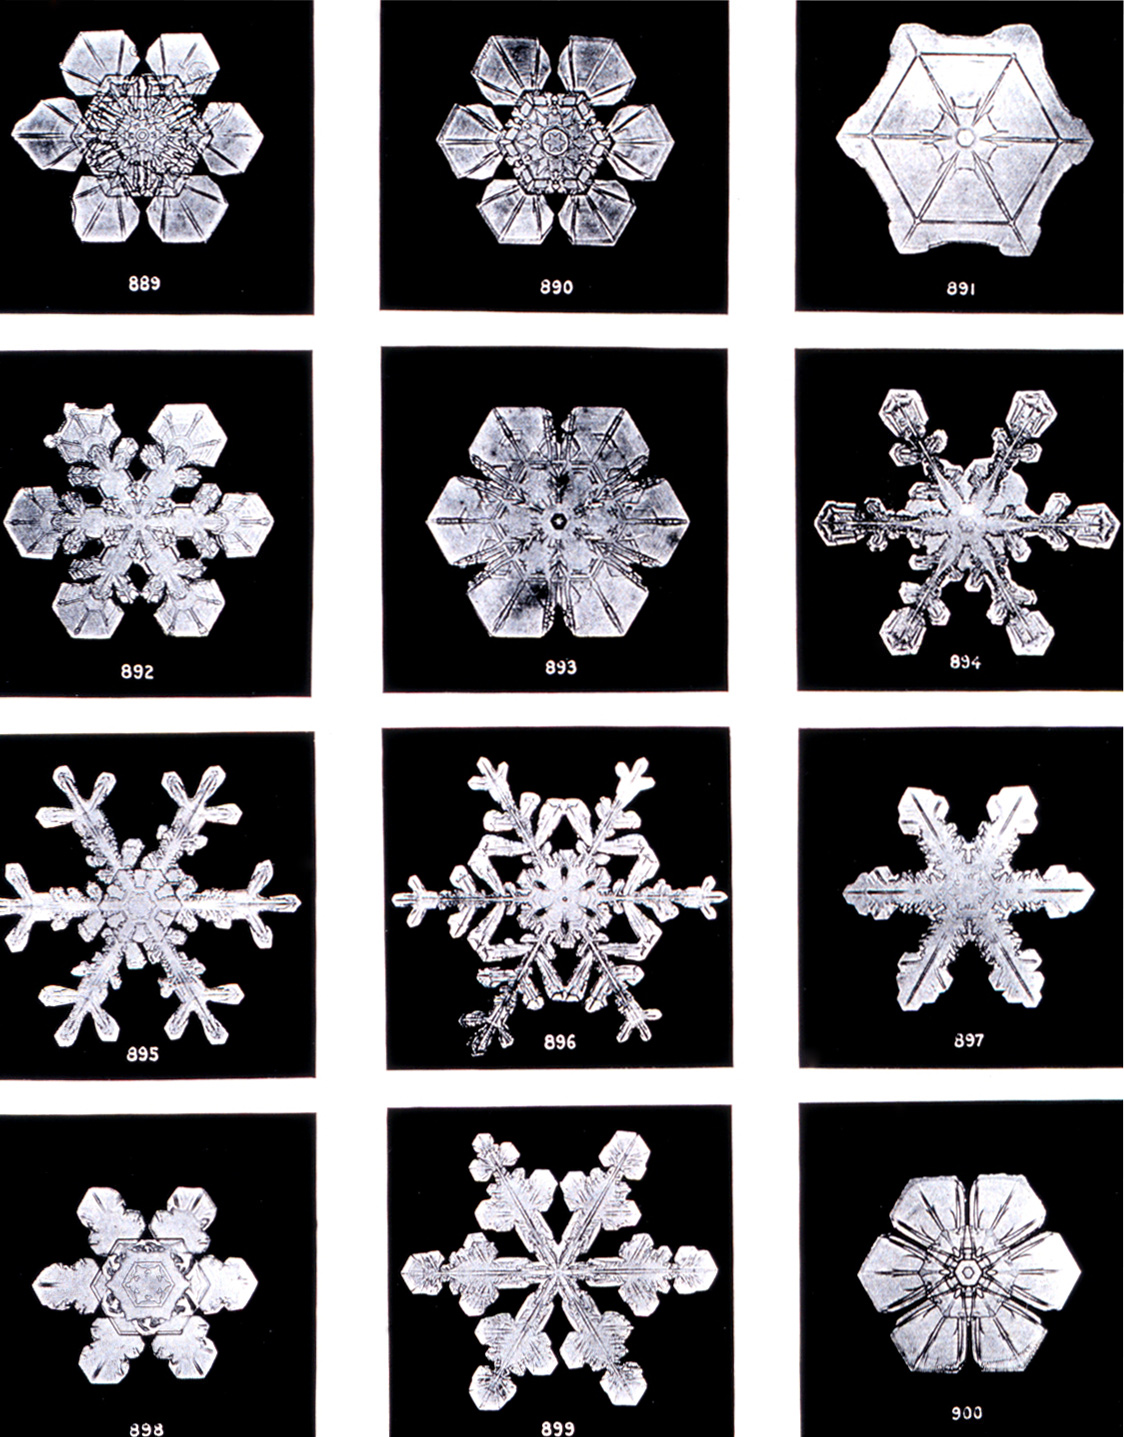
\includegraphics[width=0.36\linewidth]{images/book1/snowflakes.jpg}

{\small 1900 के दशक की शुरुआत में विल्सन बेंटली द्वारा खींचे गए हिम-क्रिस्टलों के
छायाचित्र: हर एक की छह शाखाएँ हैं।}
\end{omfigure}

\section{अभ्यास}


\begin{exercise}[$\star$]\label{exo:g11:polarity-and-cohesion:1}
आबंधों \ce{H-Cl}, \ce{O-H} और \ce{C-O} में कौन-सा \omterm{def:g7:atoms-and-molecules:atom}{परमाणु} \omterm{def:g11:polarity-and-cohesion:polar-bond}{आंशिक आवेश}
$\delta^-$ रखता है? \omterm{def:g11:polarity-and-cohesion:electronegativity}{विद्युत-ऋणात्मकताओं} की सारणी का उपयोग कीजिए।
\end{exercise}

\begin{exercise}[$\star$]\label{exo:g11:polarity-and-cohesion:2}
इनमें से कौन-से आबंध ध्रुवीय हैं: \ce{H-H}, \ce{C-H}, \ce{O-H}, \ce{N-H},
\ce{Cl-Cl}, \ce{C-Cl}? हर एक के लिए \omterm{def:g11:polarity-and-cohesion:electronegativity}{विद्युत-ऋणात्मकताओं} का अंतर
बताइए।
\end{exercise}

\begin{exercise}[$\star$]\label{exo:g11:polarity-and-cohesion:3}
हर जोड़ी में कौन-सा तत्व अधिक विद्युत-ऋणात्मक है: नाइट्रोजन या
फ़ॉस्फ़ोरस; ऑक्सीजन या सल्फ़र; कार्बन या नाइट्रोजन; सोडियम या मैग्नीशियम?
हर जोड़ी सारणी की कौन-सी प्रवृत्ति दिखाती है?
\end{exercise}

\begin{exercise}[$\star$]\label{exo:g11:polarity-and-cohesion:4}
\ce{CH4}, \ce{NH3}, \ce{H2O} और \ce{HCl} में से कौन अपने ही \omterm{def:g7:atoms-and-molecules:molecule}{अणुओं} के बीच
\omterm{def:g11:polarity-and-cohesion:hydrogen-bond}{हाइड्रोजन आबंध} बना सकता है? समझाइए।
\end{exercise}

\begin{exercise}[$\star$]\label{exo:g11:polarity-and-cohesion:5}
क्या मेथेन के \omterm{def:g11:polarity-and-cohesion:polar-molecule}{अध्रुवीय अणुओं} के बीच कोई आकर्षण होता है?
फिर भी मेथेन कमरे के ताप पर गैस क्यों है?
\end{exercise}

\begin{exercise}[$\star\star$]\label{exo:g11:polarity-and-cohesion:6}
बताइए कि हर \omterm{def:g7:atoms-and-molecules:molecule}{अणु} ध्रुवीय है या नहीं: डाइक्लोरोमेथेन \ce{CH2Cl2}
(चतुष्फलकीय), टेट्राक्लोरोमेथेन \ce{CCl4}, अमोनिया \ce{NH3}, कार्बन
डाइऑक्साइड \ce{CO2}, बोरॉन ट्राइफ़्लुओराइड \ce{BF3} (एक समतल त्रिकोण, जिसके
केंद्र में बोरॉन है)।
\end{exercise}

\begin{exercise}[$\star\star$]\label{exo:g11:polarity-and-cohesion:7}
मेथेनॉल, \ce{CH3-OH}, में कौन-सा हाइड्रोजन \omterm{def:g7:atoms-and-molecules:atom}{परमाणु} \omterm{def:g11:polarity-and-cohesion:hydrogen-bond}{हाइड्रोजन आबंध} में दिया जा सकता
है? कौन-सा \omterm{def:g7:atoms-and-molecules:atom}{परमाणु} उसे ग्रहण कर सकता है? क्या मेथेनॉल और पानी के \omterm{def:g7:atoms-and-molecules:molecule}{अणु} एक-दूसरे के
साथ \omterm{def:g11:polarity-and-cohesion:hydrogen-bond}{हाइड्रोजन आबंध} बना सकते हैं? एक बनाइए।
\end{exercise}

\begin{exercise}[$\star\star$]\label{exo:g11:polarity-and-cohesion:8}
समझाइए कि क्वथन ताप \ce{CH4} <
\ce{SiH4} < \ce{GeH4} के क्रम में क्यों बढ़ते हैं।
\end{exercise}

\begin{exercise}[$\star\star$]\label{exo:g11:polarity-and-cohesion:9}
हाइड्राइडों के क्वथन तापों वाले चार्ट पर कौन-सा समूह अपने पहले सदस्य के लिए कोई
असामान्य मान नहीं दिखाता? क्यों?
\end{exercise}

\begin{exercise}[$\star\star$]\label{exo:g11:polarity-and-cohesion:10}
% ledger: en:H, en:Cl, en:Br, en:I, bp:HCl, bp:HBr, bp:HI
आबंध \ce{H-Cl}, \ce{H-Br}, \ce{H-I} उत्तरोत्तर कम ध्रुवीय हैं (क्लोरीन,
ब्रोमीन और आयोडीन की \omterm{def:g11:polarity-and-cohesion:electronegativity}{विद्युत-ऋणात्मकताएँ} 3.16, 2.96 और
2.66 हैं), फिर भी क्वथन ताप बढ़ते हैं: \qty{-85}{\celsius},
\qty{-66}{\celsius}, \qty{-35}{\celsius}। कौन-सी अन्योन्यक्रिया हावी है, और
क्यों?
\end{exercise}

\begin{exercise}[$\star\star$]\label{exo:g11:polarity-and-cohesion:11}
कमरे के ताप पर क्लोरीन गैस है और आयोडीन ठोस, हालाँकि दोनों
\omterm{def:g11:polarity-and-cohesion:polar-molecule}{अध्रुवीय अणुओं} \ce{X2} से बने हैं। समझाइए।
\end{exercise}

\begin{exercise}[$\star\star\star$]\label{exo:g11:polarity-and-cohesion:12}
% ledger: bp:C2H5OH, bp:CH3OCH3, bp:C3H8
एथेनॉल \ce{CH3-CH2-OH}, मेथॉक्सीमेथेन \ce{CH3-O-CH3} और प्रोपेन
\ce{CH3-CH2-CH3} का \omterm{def:g10:the-mole:molar-mass}{मोलर द्रव्यमान} लगभग एक ही है। वे
\qty{78}{\celsius}, \qty{-25}{\celsius} और \qty{-42}{\celsius} पर उबलते हैं। इनमें से
कौन ध्रुवीय हैं? कौन अपने ही \omterm{def:g7:atoms-and-molecules:molecule}{अणुओं} के बीच \omterm{def:g11:polarity-and-cohesion:hydrogen-bond}{हाइड्रोजन आबंध} बनाते हैं? क्रम
समझाइए।
\end{exercise}

\begin{exercise}[$\star\star\star$]\label{exo:g11:polarity-and-cohesion:13}
बर्फ़ में पानी का हर \omterm{def:g7:atoms-and-molecules:molecule}{अणु} चार पड़ोसियों से हाइड्रोजन आबंधित होता है, एक
खुले जाल में; द्रव पानी में जाल टूटता रहता है और आंशिक रूप से
ढह जाता है। समझाइए कि बर्फ़ पानी पर क्यों तैरती है। जमी हुई झील की मछलियों के लिए
यह क्यों महत्वपूर्ण है?
\end{exercise}

\begin{exercise}[$\star\star\star$]\label{exo:g11:polarity-and-cohesion:14}
गलन ताप के बढ़ते क्रम में लगाइए, और कणों के बीच के आकर्षणों से
पुष्टि कीजिए: पोटैशियम क्लोराइड \ce{KCl}, बर्फ़
\ce{H2O}, ठोस मेथेन \ce{CH4}।
\end{exercise}

\begin{exercise}[$\star\star\star$]\label{exo:g11:polarity-and-cohesion:15}
% ledger: en:F, en:O, bp:HF, bp:H2O
फ़्लुओरीन ऑक्सीजन से अधिक विद्युत-ऋणात्मक है, इसलिए \ce{H-F} आबंध
\ce{O-H} आबंध से अधिक ध्रुवीय है। फिर भी पानी \qty{100}{\celsius} पर उबलता है
और हाइड्रोजन फ़्लुओराइड \qty{20}{\celsius} पर। गिनिए कि हर \omterm{def:g7:atoms-and-molecules:molecule}{अणु} कितने हाइड्रोजन
\omterm{def:g7:atoms-and-molecules:atom}{परमाणु} दे सकता है और कितने \omterm{def:g10:lewis-and-shape:lone-pair}{एकाकी युग्मों} से ग्रहण कर सकता है, और
समझाइए।
\end{exercise}

\section{समस्या: पानी \texorpdfstring{\qty{100}{\celsius}}{100 डिग्री सेल्सियस} पर क्यों उबलता है?}

\begin{problem}[{सप्ताहांत समस्या --- हाइड्रोजन आबंधों के बिना पानी किस
ताप पर उबलता?}]
\label{pb:g11:polarity-and-cohesion:1}
% ledger: en:H, en:O, en:S, en:Se, bp:H2O, bp:H2S, bp:H2Se, bp:CH4, bp:SiH4, bp:GeH4, bp:HCl, bp:HBr, bp:HF, bp:NH3, bp:PH3, bp:AsH3
ऑक्सीजन, सल्फ़र और सेलेनियम सारणी के एक ही समूह में हैं, और तीनों
हाइड्रोजन के साथ एक यौगिक बनाते हैं: \ce{H2O}, \ce{H2S}, \ce{H2Se}।
हाइड्राइडों के हर समूह में क्वथन ताप आम तौर पर \omterm{def:g7:atoms-and-molecules:molecule}{अणु} के आकार के साथ
बढ़ते हैं। पानी इस नियम को तोड़ता है। कितना?

\medskip
\noindent\textbf{भाग I --- तीन \omterm{def:g7:atoms-and-molecules:molecule}{अणु}।}
\begin{enumerate}
  \item \ce{H2O}, \ce{H2S} और \ce{H2Se} की \omterm{def:g10:lewis-and-shape:lewis-structure}{लुइस संरचनाएँ} बनाइए।
        वे एक जैसी क्यों हैं?
  \item उनके \omterm{def:g10:the-mole:molar-mass}{मोलर द्रव्यमान} निकालिए।
  \item आबंधों \ce{O-H}, \ce{S-H} और \ce{Se-H} के \omterm{def:g11:polarity-and-cohesion:electronegativity}{विद्युत-ऋणात्मकता}
        अंतर निकालिए (ऑक्सीजन 3.44, सल्फ़र 2.58,
        सेलेनियम 2.55, हाइड्रोजन 2.20)। कौन-से आबंध स्पष्ट रूप से ध्रुवीय हैं?
  \item तीनों \omterm{def:g7:atoms-and-molecules:molecule}{अणुओं} की आकृति क्या है? क्या वे ध्रुवीय हैं?
  \item हर \omterm{def:g7:atoms-and-molecules:molecule}{अणु} के \omterm{def:g9:inside-the-atom:nucleus}{इलेक्ट्रॉन} गिनिए। किसकी \omterm{def:g11:polarity-and-cohesion:van-der-waals}{वान्डरवाल्स
        अन्योन्यक्रियाएँ} सबसे प्रबल हैं?
\end{enumerate}

\medskip
\noindent\textbf{भाग II --- \omterm{def:g11:polarity-and-cohesion:hydrogen-bond}{हाइड्रोजन आबंध}।}
\begin{enumerate}[resume]
  \item तीनों में से कौन-सा यौगिक अपने \omterm{def:g7:atoms-and-molecules:molecule}{अणुओं} के बीच \omterm{def:g11:polarity-and-cohesion:hydrogen-bond}{हाइड्रोजन आबंध} बनाता
        है? बाकी क्यों नहीं?
  \item पानी का एक \omterm{def:g7:atoms-and-molecules:molecule}{अणु} अधिक से अधिक कितने \omterm{def:g11:polarity-and-cohesion:hydrogen-bond}{हाइड्रोजन आबंधों} में भाग ले
        सकता है? उन्हें बनाइए।
  \item द्रव में हाइड्रोजन सल्फ़ाइड के \omterm{def:g7:atoms-and-molecules:molecule}{अणुओं} को कौन-सी अन्योन्यक्रियाएँ
        जोड़े रखती हैं?
\end{enumerate}

\medskip
\noindent\textbf{भाग III --- प्रवृत्ति।}
\begin{enumerate}[resume]
  \item हाइड्रोजन सल्फ़ाइड \qty{212.9}{K} पर उबलता है और हाइड्रोजन सेलेनाइड
        \qty{-41.3}{\celsius} पर। पहले वाले को डिग्री सेल्सियस में व्यक्त कीजिए
        ($\theta = T - 273.15$)।
  \item \omterm{def:g9:periodic-table-first-look:period}{आवर्त} 3 (\ce{H2S}) से \omterm{def:g9:periodic-table-first-look:period}{आवर्त} 4 (\ce{H2Se}) तक क्वथन ताप कितना
        बढ़ता है?
  \item यह क्यों बढ़ता है?
  \item \omterm{def:g9:periodic-table-first-look:period}{आवर्त} 2 से \omterm{def:g9:periodic-table-first-look:period}{आवर्त} 3 तक भी उतनी ही वृद्धि मानकर, एक ``सामान्य'' \ce{H2O}
        किस ताप पर उबलता?
  \item इस विधि को \omterm{def:g9:periodic-table-first-look:period}{समूह} 14 पर परखिए: \ce{SiH4} \qty{-112}{\celsius} पर
        और \ce{GeH4} \qty{-88.1}{\celsius} पर उबलता है।
        \ce{CH4} के क्वथन ताप का अनुमान लगाइए और उसकी तुलना वास्तविक मान,
        \qty{-162}{\celsius}, से कीजिए। क्या बहिर्वेशन सटीक है?
  \item यही \omterm{def:g9:periodic-table-first-look:period}{समूह} 17 के लिए कीजिए (\ce{HCl} \qty{-85.1}{\celsius},
        \ce{HBr} \qty{-66.4}{\celsius}) और \ce{HF},
        \qty{19.6}{\celsius}, से तुलना कीजिए।
\end{enumerate}

\medskip
\noindent\textbf{भाग IV --- अंतर।}
\begin{enumerate}[resume]
  \item पानी वास्तव में \qty{100}{\celsius} पर उबलता है। वास्तविक और बहिर्वेशित
        मानों के बीच का अंतर कितना बड़ा है?
  \item यही अमोनिया के लिए, \ce{PH3} \qty{-87.8}{\celsius} और
        \ce{AsH3} \qty{-62.5}{\celsius} का उपयोग करके; अमोनिया वास्तव में
        \qty{-33.4}{\celsius} पर उबलती है।
  \item पानी, हाइड्रोजन फ़्लुओराइड और अमोनिया को उनके अंतर के आकार के अनुसार
        क्रम दीजिए, और \omterm{def:g11:polarity-and-cohesion:hydrogen-bond}{हाइड्रोजन आबंध} गिनकर इस क्रम को समझाइए।
  \item \omterm{def:g11:polarity-and-cohesion:hydrogen-bond}{हाइड्रोजन आबंधों} के बिना क्या पानी कमरे के ताप पर ठोस, द्रव या गैस
        होता? पृथ्वी के लिए इसका क्या अर्थ होता?
  \item प्रश्न 12 का उत्तर केवल एक अनुमान क्यों है?
  \item अंतिम उत्तर बताइए: \omterm{def:g11:polarity-and-cohesion:hydrogen-bond}{हाइड्रोजन आबंधों} के बिना पानी लगभग किस ताप पर
        उबलता?
\end{enumerate}
\end{problem}
